\documentclass[a4paper]{article}
\usepackage{polski}
\usepackage[cp1250]{inputenc}
\usepackage{url}
\usepackage{hyperref}
\usepackage{graphicx}

\title{\vspace{3cm} \bf{\Huge Internetowy\\ \vspace{0.2cm} Serwis\\ \vspace{0.4cm} Aukcyjny}}
\author{{\em Jakub Niewczas, Damian Klimek, Tomasz Zabrzewski, Łukasz Myszkowski}}
\date{}

\begin{document}
	
	\begin{titlepage}
		\thispagestyle{empty}
		\maketitle
		\vspace{8cm}
		\begin{center}
			Zespołowe przedsięwzięcie inżynierskie\\[2mm]
			
			Informatyka\\[2mm]
			
			Rok. akad. 2017/2018, sem. I\\[2mm]
			
			Prowadzący: dr hab. Marcin Mazur
		\end{center}
	\end{titlepage}
	
	\tableofcontents
	\thispagestyle{empty}
	
	\newpage
	
	\section{Opis projektu}
	
	\subsection{Członkowie zespołu}
	
	\begin{enumerate}
		\item Damian Klimek (kierownik projektu);
		\item Jakub Niewczas;
		\item Tomasz Zabrzewski;
		\item Łukasz Myszkowski;
	\end{enumerate}
	
	\subsection{Cel projektu (produkt)}
	
	Głównym i najważniejszym celem projektu jest stworzenie platformy webowej, która pojęcie ,,zakupy'' pchnie krok dalej. Potencjalni klienci będą mieć możliwość robienia zakupów \emph{(tj. sprzedawanie i kupowanie przedmiotów)} bez wychodzenia z domu. Kolejną ważną rzeczą jest zaimplementowanie modułu indywidualnych kont dla użytkowników \emph{(logowanie się na swoje konto oraz rejestrowanie nowego)}. Również stawiamy nacisk na stworzenie miłego dla oka, prostego a przede wszystkim intuicyjnego designu strony internetowej aby użytkownicy mogli w łatwy sposób przemieszczać się po platformie i szybko wyszukiwać interesujące ich przedmioty.
	
	\subsection{Potencjalny odbiorca produktu (klient)}
	
	Konkretnym klientem może być każdy, kto potrzebuje pieniędzy przez co dostaje możliwość sprzedania czegokolwiek lub osoby potrzebujące jakiegoś dobra. Widełki wieku klientów nie są definiowalne - każdy kto posiada dostęp do internetu może skorzystać z usług jakie oferuje produkt.
	
	\subsection{Metodyka}
	
	Projekt będzie realizowany przy użyciu (zaadaptowanej do istniejących warunków) metodyki {\em Scrum}. 
	
	\section{Wymagania użytkownika}
	
	\subsection{User story 1}
	Jako nowy użytkownik serwisu chciałbym mieć możliwość założenia swojego indywidualnego konta, żebym mógł korzystać w pełni z usług dostarczanych przez serwis.
	
	\subsection{User story 2}
	Jako użytkownik chciałbym mieć możliwość zalogować się na swoje indywidualne konto, by móc korzystać z wszystkich usług platformy.
	
	\subsection{User story 3}
	Jako użytkownik chciałbym mieć możliwość wystawienia przedmiotu na aukcję, żebym mógł sprzedawać przedmioty oraz zarabiać pieniądze.
	
	\subsection{User story 4}
	Jako użytkownik podczas wystawiania przedmiotu na aukcję chciałbym mieć możliwość wybrania formy aukcji \emph{(tj. licytacja, opcja ,,KUP TERAZ'' lub obie formy)}, żebym mógł sprzedać przedmiot w wybranej formie aukcji.
	
	\subsection{User story 5}
	Jako użytkownik podczas wystawiania przedmiotu na aukcję chciałbym mieć możliwość wprowadzenia opisu aukcji:
	\begin{itemize}
		\item konkretna nazwa aukcji;
		\item dodatkowe informację o sprzedawanym przedmiocie;
		\item cena \emph{(wywoławcza podczas licytacji lub stała za przedmiot podczas opcji ,,KUP TERAZ'')};
		\item wgranie zdjęcia przedmiotu;
	\end{itemize}
	żebym mógł zachęcić potencjalnego kupca do zakupu przedmiotu.
	
	\subsection{User story 6 (Opcjonalnie)}
	Jako użytkownik chciałbym mieć możliwość komentowania produktów innych osób wystawiających przedmioty na aukcji, , żebym mógł dowiedzieć się interesujących informacji od innych osób, które wcześniej kupiły przedmiot na jego temat bądź podzielić się własną opinią. 
	
	\subsection{User story 7}
	Jako użytkownik chciałbym mieć możliwość dodania przedmiotów które mnie interesują do zakładek \emph{ (tj. Ulubione)}, żebym mógł szybko i łatwo je odnaleźć. 
	
	\subsection{User story 8}
	Jako użytkownik chciałbym mieć możliwość dodania swoich danych:
	\begin{itemize}
		\item imię;
		\item nazwisko;
		\item miejscowość;
		\item numer telefonu;
		\item e-mail;
		\item numer konta bankowego;
	\end{itemize}
	żeby umożliwić innym użytkownikom kontakt ze mną i rozliczeń.
	
	\subsection{User story 9}
	Jako użytkownik chciałbym mieć możliwość zmiany:
	\begin{itemize}
		\item istniejącego  hasła na nowe;
		\item istniejącego e-maila na nowy;
		\item danych osobowe na nowe;
	\end{itemize}
	żeby zaktualizować email oraz wprowadzić nowe hasło bądź też poprawić błąd w danych osobowych lub całkowicie je zmienić.
	
	\subsection{User story 10}
	Jako użytkownik chciałbym mieć możliwość zobaczenia ile razy odwiedzono moją aukcję \emph{ (tj. licznik odsłon)}, żebym mógł zobaczyć jakie jest zainteresowanie moją aukcją.
	
	\subsection{User story 11}
	Jako użytkownik chciałbym mieć możliwość edytowania danych aukcji \emph{ (tj. cena, opis)} oraz usunięcia danej aukcji, żebym mógł poprawić błedy lub zaktualizować dane aukcji.
	
	\subsection{User story 12}
	Jako użytkownik chciałbym mieć możliwość wyszukiwania interesujących mnie aukcji poprzez podanie słów kluczowych w wyszukiwarce, żebym mógł znaleźć przedmiot, który chciałbym zakupić.
	
	\subsection{User story 13}
	Jako użytkownik chciałbym by po dokonaniu transakcji (kup teraz bądź wygrana licytacja) wysyłała się do kupującego wiadomość z moim numerem konta oraz informacjami dotyczącymi transakcji, by mógł on dokonać wpłaty za zakupiony przedmiot.
	
	\subsection{User story 14}
	Jako użytkownik chciałbym mieć możliwość sprawdzenia starych aukcji które zostały zakończone (przedmiot sprzedano, przedmiot kupiono) bądź też wygasły, żebym mógl sprawdzić historie swoich transakcji.
	 
	\subsection{User story 15}
	Jako użytkownik chciałbym mieć możliwość wysłania wiadomości prywatnej do innego użytkownika serwisu, żebym mógł się z nim skontaktować. 
	
	\subsection{User story 16}
	Jako użytkownik chciałbym mieć możliwość przeglądania wszystkich dostępnych aukcji na serwisie w postaci listy wraz z ich podstawowymi danymi \emph{(tj. nazwa aukcji, forma aukcji, cena, data rozpoczęcia oraz zakończenia aukcji)}, żebym mógł przeglądać aukcje oferowane przez serwis.
	
	\subsection{User story 17}
	Jako użytkownik chciałbym mieć możliwość zakupu produktu natychmiast (opcja kup teraz), bądź licytowania go (opcja licytuj), żebym mógł go kupić.
	
	\subsection{User story 18}
	Jako użytkownik chciałbym mieć możliwość posiadania paska nawigacyjnego w którym zostanie umiejscowiona wyszukiwarka, oraz panel konta użytkownika.
		
	\section{Harmonogram}
	
	\subsection{Rejestr zadań (Product Backlog)}
	
		\begin{itemize}
		\item Data rozpoczęcia: 24.10.2017;
		\item  Data zakończenia: 31.10.2017;
	\end{itemize}
	
	\subsection{Sprint 1}
	
	\begin{itemize}
		\item Data rozpoczęcia: \emph{31.10.2017};
		\item Data zakończenia: \emph{14.11.2017};
		\item Scrum Master: \emph{Łukasz Myszkowski};
		\item Product Owner: \emph{Tomasz Zabrzewski};
		\item Development Team: \emph{Jakub Niewczas, Damian Klimek, Łukasz Myszkowski};
	\end{itemize}
	
	\subsection{Sprint 2}
	
	\begin{itemize}
		\item Data rozpoczęcia: \emph{14.11.2017};
		\item  Data zakończenia: \emph{28.11.2017};
		\item Scrum Master: \emph{Tomasz Zabrzewski};
		\item Product Owner: \emph{Damian Klimek};
		\item Development Team: \emph{Łukasz Myszkowski, Jakub Niewczas, Damian Klimek};
	\end{itemize}

	\subsection{Sprint 3}

	\begin{itemize}
		\item Data rozpoczęcia: \emph{28.11.2017};
		\item  Data zakończenia: \emph{12.12.2017};
		\item Scrum Master: \emph{Damian Klimek};
		\item Product Owner: \emph{Jakub Niewczas};
		\item Development Team: \emph{Tomasz Zabrzewski, Łukasz Myszkowski, Jakub Niewczas};
	\end{itemize}
	
	\subsection{Sprint 4}

	\begin{itemize}
		\item Data rozpoczęcia: \emph{12.12.2017};
		\item  Data zakończenia: \emph{09.01.2018};
		\item Scrum Master: \emph{Jakub Niewczas};
		\item Product Owner: \emph{Damian Klimek};
		\item Development Team: \emph{Tomasz Zabrzewski, Łukasz Myszkowski, Damian Klimek};
	\end{itemize}

	\subsection{Sprint 5}

	\begin{itemize}
		\item Data rozpoczęcia: \emph{09.01.2018};
		\item  Data zakończenia: \emph{23.01.2018};
		\item Scrum Master: \emph{Łukasz Myszkowski};
		\item Product Owner: \emph{Tomasz Zabrzewski};
		\item Development Team: \emph{Damian Klimek, Jakub Niewczas, Tomasz Zabrzewski};
	\end{itemize}
	
	\section{Product Backlog}
	
	\subsection{Backlog Item 1}
	\paragraph{Tytuł zadania:} Baza danych
	\paragraph{Opis zadania:} Przygotowanie struktury bazy danych.
	\paragraph{Priorytet:} Wysoki
	\paragraph{Definition of Done:} Baza danych powinna zawierać tyle tabel ile potrzeba na stworzenie aplikacji. Środowisko bazodanowe \textbf{MySQL}. Baza danych serwisu musi posiadać następujące struktury.
	\vspace{0.5cm}
	\\Struktura tabeli \textbf{users}:
	\begin{itemize}
		\item \textbf{id} $\to$ [typ - \verb|INT|, \verb|AUTO_INCREMENT|];
		\item \textbf{username} $\to$ [typ - \verb|VARCHAR(32)|, kodowanie - \verb|UTF8_GENERAL_CI|];
		\item \textbf{password} $\to$ [typ - \verb|VARCHAR(32)|, kodowanie - \verb|UTF8_GENERAL_CI|];
		\item \textbf{firstname} $\to$ [typ - \verb|VARCHAR(64)|, kodowanie - \verb|UTF8_GENERAL_CI|];
		\item \textbf{surname} $\to$ [typ - \verb|VARCHAR(64)|, kodowanie - \verb|UTF8_GENERAL_CI|];
		\item \textbf{email} $\to$ [typ - \verb|VARCHAR(64)|, kodowanie - \verb|UTF8_GENERAL_CI|];
		\item \textbf{phone} $\to$ [typ - \verb|VARCHAR(9)|, kodowanie - \verb|UTF8_GENERAL_CI|];
		\item \textbf{place} $\to$ [typ - \verb|VARCHAR(128)|, kodowanie - \verb|UTF8_GENERAL_CI|];
		\item \textbf{bank} $\to$ [typ - \verb|VARCHAR(26)|, kodowanie - \verb|UTF8_GENERAL_CI|];
		\item \textbf{avatar} $\to$ [typ - \verb|VARCHAR(128)|, kodowanie - \verb|UTF8_GENERAL_CI|];
	\end{itemize}

	\vspace{0.5cm}
	Struktura tabeli \textbf{categories}:
	\begin{itemize}
		\item \textbf{id} $\to$ [typ - \verb|INT|, \verb|AUTO_INCREMENT|];
		\item \textbf{name} $\to$ [typ - \verb|VARCHAR(64)|, kodowanie - \verb|UTF8_GENERAL_CI|];
	\end{itemize}

	\vspace{0.5cm}
	Struktura tabeli \textbf{auctions}:
	\begin{itemize}
		\item \textbf{id} $\to$ [typ - \verb|INT|, \verb|AUTO_INCREMENT|];
		\item \textbf{name} $\to$ [typ - \verb|VARCHAR(128)|, kodowanie - \verb|UTF8_GENERAL_CI|];
		\item \textbf{category} $\to$ [typ - \verb|INT|, relacja z kolumną id z tabeli categories];
		\item \textbf{buy\_prize} $\to$ [typ - \verb|VARCHAR(16)|, kodowanie - \verb|UTF8_GENERAL_CI|];
		\item \textbf{bidding\_prize} $\to$ [typ - \verb|VARCHAR(16)|, kodowanie - \verb|UTF8_GENERAL_CI|];
		\item \textbf{description} $\to$ [typ - \verb|VARCHAR(512)|, kodowanie - \verb|UTF8_GENERAL_CI|];
		\item \textbf{image} $\to$ [typ - \verb|VARCHAR(256)|, kodowanie - \verb|UTF8_GENERAL_CI|];
		\item \textbf{last\_bidder} $\to$ [typ - \verb|INT|, relacja z kolumną id z tabeli users];
		\item \textbf{buyer} $\to$ [typ - \verb|INT|, relacja z kolumną id z tabeli users];
	\end{itemize}

	\vspace{0.5cm}
	Struktura tabeli \textbf{comments}:
	\begin{itemize}
		\item \textbf{id} $\to$ [typ - \verb|INT|, \verb|AUTO_INCREMENT|];
		\item \textbf{message} $\to$ [typ - \verb|VARCHAR(512)|, kodowanie - \verb|UTF8_GENERAL_CI|];
		\item \textbf{owner} $\to$ [typ - \verb|INT|, relacja z kolumną id z tabeli users];
		\item \textbf{auction} $\to$ [typ - \verb|INT|, relacja z kolumną id z tabeli auctions];
	\end{itemize}

	\vspace{0.5cm}
	Struktura tabeli \textbf{messages}:
	\begin{itemize}
		\item \textbf{id} $\to$ [typ - \verb|INT|, \verb|AUTO_INCREMENT|];
		\item \textbf{owner} $\to$ [typ - \verb|INT|, relacja z kolumną id z tabeli users];
		\item \textbf{recipient} $\to$ [typ - \verb|INT|, relacja z kolumną id z tabeli users];
		\item \textbf{title} $\to$ [typ - \verb|VARCHAR(128)|, kodowanie - \verb|UTF8_GENERAL_CI|];
		\item \textbf{message} $\to$ [typ - \verb|VARCHAR(512)|, kodowanie - \verb|UTF8_GENERAL_CI|];
		\item \textbf{readed} $\to$ [typ - \verb|INT|];
	\end{itemize} 
	
	\subsection{Backlog Item 2}
	\paragraph{Tytuł zadania:} Rejestracja
	\paragraph{Opis zadania:} Możliwość założenia nowego konta;
	\paragraph{Priorytet:} Wysoki
	\paragraph{Definition of Done:} Każda osoba powinna mieć możliwość założenia swojego indywidualnego konta. Należy stworzyć formularz z podstawowymi danymi (\emph{tj. login, hasło, imię, nazwisko, e-mail, miejscowość, numer telefonu, numer konta bankowego oraz avatar}). Wpisane przez użytkownika dane muszą być pobierane metodą \emph{POST}. Finalnym efektem rejestracji jest wysłanie zapytania do bazy danych, który utworzy nowy rekord w tabeli \emph{users} z danymi użytkownika.
	
	\subsection{Backlog Item 3}
	\paragraph{Tytuł zadania:} Zabezpieczenie hasła
	\paragraph{Opis zadania:} Wymuszenie od użytkownika wprowadzenia danych spełniających określone kryteria;
	\paragraph{Priorytet:} Niski
	\paragraph{Definition of Done:} Użytkownik tworzący nowe konto musi podać hasło składające się z minimum 8 znaków w tym:
	\begin{itemize}
		\item wielkie litery od A do Z;
		\item małe litery od a do z;
		\item cyfry od 0 do 9;
		\item znaki niealfabetyczne (np. \verb|!, @, #, &|);
	\end{itemize}
	Należy stworzyć skrypt używający \emph{wyrażenia regularne}, które w łatwy sposób mogą sprawdzić poprawność hasła z wyżej ustalonymi zasadami. Hasło, które będzie podawał użytkownik rejestrując lub logując się na swoje konto powinno być niewidoczne dla osób postronnych (wykropkowane).

	\subsection{Backlog Item 4}
	\paragraph{Tytuł zadania:} Weryfikowanie danych
	\paragraph{Opis zadania:} Sprawdzanie wprowadzanych danych przez użytkownika podczas rejestracji;
	\paragraph{Priorytet:} Wysoki
	\paragraph{Definition of Done:} Każda osoba wprowadzająca dane do serwisu podczas rejestracji powinna podać poprawne dane:
	\begin{itemize}
		\item imię - powinno zawierać od 3 do 32 znaków, w tym tylko od a do z;
		\item nazwisko - powinno zawierać od 3 do 32 znaków, w tym tylko od a do z;
		\item e-mail - powinien przypominać maskę (tj. mójemail09@domena.pl);
		\item miejscowość - powinna zawierać od 3 do 64 znaków, w tym tylko od a do z;
		\item numer telefonu - powinna składać się z 9 cyfr.
		\item konto bankowe - powinno składać się z 26 cyfr.	
	\end{itemize}
	Gdy użytkownik nie zastosuje się do wyżej wymienionych zasad, należy wysłać do niego w postaci \emph{JavaScript Popup Alert box}, wiadomość zwrotną podającą, w którym miejscu popełnił błąd oraz jak poprawnie wypełnić input formularza.
	
	\subsection{Backlog Item 5}
	\paragraph{Tytuł zadania:} Logowanie
	\paragraph{Opis zadania:} Możliwość zalogowania się na swoje konto;
	\paragraph{Priorytet:} Wysoki
	\paragraph{Definition of Done:} Stworzenie formularza logowania (tj. login oraz hasło) pobierające owe dane, następnie w postaci zapytania MySQL musi sprawdzać czy istnieją dane w bazie danych oraz czy pasują do jednego użytkownika. Należy zaimplementować wiadomość zwrotną gdy użytkownik wpisał złe dane (nie ma takiego rekordu w bazie danych bądź hasło nie pasuje do loginu). Po udanej operacji (logowanie powiodło się) należy stworzyć użytkownikowi sesję oraz przekierować go na stronę główną serwisu.
	
	\subsection{Backlog Item 6}
	\paragraph{Tytuł zadania:} Pasek nawigacji
	\paragraph{Opis zadania:} Utworzenie paska nawigacji umieszczonego w górnej części ekranu;
	\paragraph{Priorytet:} Wysoki
	\paragraph{Definition of Done:} Należy utworzyć pasek nawigacji, który będzie umiejscowiony na górze ekranu przeglądarki. Pozycjonowanie paska należy ustawić jako \emph{fixed}, aby w przypadku długiej strony ,,przykleił'' się do ekranu i podążał za scrollowaną stroną. Szerokość paska powinna być uzależniona od szerokości ekranu, na którym będzie odwiedzany serwis, zaś wysokość powinna być ustawiona na \emph{75px}.
	
	\subsection{Backlog Item 7}
	\paragraph{Tytuł zadania:} Zmiana danych
	\paragraph{Opis zadania:} Umożliwienie użytkownikowi zmiany swoich podstawowych danych;
	\paragraph{Priorytet:} Średni
	\paragraph{Definition of Done:} Każda osoba posiadająca swoje konto powinna mieć możliwość zmiany swoich podstawowych danych na nowe (tj. imię, nazwisko, e-mail, miejscowość, numer telefonu, numer konta bankowego, hasło oraz avatar). Należy stworzyć formularz z wcześniej wymienionymi danymi oraz jako domyślne \emph{value} kolejnych inputów formularza powinny być przypisane dane pobrane z bazy danych. Obowiązkowo należy zaimplementować przycisk \emph{submit}, po kliknięciu którego zostaną pobrane dane z formularza metodą \emph{POST} oraz wysłane do bazy danych w postaci zapytania MySQL. Wysłane dane muszą podmieniać już istniejące.
	
	\subsection{Backlog Item 8}
	\paragraph{Tytuł zadania:} Wyszukiwarka
	\paragraph{Opis zadania:} Umożliwienie użytkownikowi wyszukiwania interesujących przedmiotów;
	\paragraph{Priorytet:} Średni
	\paragraph{Definition of Done:} Każda osoba (zalogowana lub niezalogowana) może używać wyszukiwarki. Wyszukiwarke w postaci formularza należy umieścić na pasku nawigacji, który znajduje się na górze ekranu. Wpisane hasło w input formularza zwrócone przez funkcję \emph{htmlspecialchars()} należy umieścić w zapytaniu MySQL w poszukiwaniu przedmiotów. Zapytanie należy zaprojektować tak, aby wyszukiwał każdy przedmiot, w którym zawiera się wpisane przez użytkownika hasło \emph{(np. dom, domek, domeczek, domuś itp.)}.
	
	\subsection{Backlog Item 9}
	\paragraph{Tytuł zadania:} Panel konta
	\paragraph{Opis zadania:} Zgrupowanie w jedno miejsce podstawowych akcji użytkownika;
	\paragraph{Priorytet:} Średni
	\paragraph{Definition of Done:} Panel należy podzielić na dwie grupy - dla osób zalogowanych oraz dla osób niezalogowanych. Oba panele powinny być umiejscowione na pasku nawigacji na górze ekranu. Panel dla zalogowanego użytkownika powinien być w postaci avataru użytkownika, w który można kliknąć a następnie rozwija się menu z podstawowymi akcjami \emph{(tj. edytuj dane, moje aukcje, historia zakupów, wyloguj)}. Panel dla osoby niezalogowanej powinien być w postaci napisu ,,Moje konto'', które również rozwija się po kliknięciu w napis, z którego można wybrać dwie akcję \emph{(tj. zarejestruj się, zaloguj się)}. Po kliknięciu, w któryś z odnośników z rozwijanych menu każdy powinien być przekierowywany na konkretne podstrony serwisu.
	
	\subsection{Backlog Item 10}
	\paragraph{Tytuł zadania:} Dodanie aukcji
	\paragraph{Opis zadania:} Umożliwienie użytkownikowi wystawienia nowej aukcji;
	\paragraph{Priorytet:} Wysoki
	\paragraph{Definition of Done:} Każda osoba zalogowana na swoję konto powinna mieć tę opcję dostępną. Osoba, która nie jest zalogowana na swoje konto powinna dostać wiadomość zwrotną, że ta opcja jest tylko dla osób zalogowanych lub całkowicie zablokować dostęp. Tworzenie nowego rekordu w bazie danych w tabeli \emph{auction}.
	
	\subsection{Backlog Item 11}
	\paragraph{Tytuł zadania:} Formularz aukcyjny
	\paragraph{Opis zadania:} Umożliwienie użytkownikowi podanie niezbędnych danych dotyczących aukcji;
	\paragraph{Priorytet:} Wysoki
	\paragraph{Definition of Done:} Osoba zalogowana podczas wystawiania nowego przedmiotu na akcję musi mieć możliwość wpisania niezbędnych danych, które pozwolą odróżniać od siebie inne aukcje (tj. konkretna nazwa aukcji, opis przedmiotu, cena, zdjęcie). Formularz powinien pobierać dane metodą \emph{POST}.
	
	\subsection{Backlog Item 12}
	\paragraph{Tytuł zadania:} Edytowanie aukcji
	\paragraph{Opis zadania:} Umożliwienie użytkownikowi edytowania danych swojej aukcji;
	\paragraph{Priorytet:} Średni
	\paragraph{Definition of Done:} Użytkownik, który wystawił przedmiot na aukcję powinien mieć możliwość edytowania danych związanych z aukcją. Należy stworzyć formularz, w którym domyślnymi wartościami kolejnych inputów będą dane wczytane z bazy danych. Dane z formularza powinny być pobierane metodą \emph{POST}. Kliknięcie przycisku \emph{submit} skutować powinno nadpisanie istniejących danych w bazie poprzez wykonanie zapytania \emph{UPDATE}.
	
	\subsection{Backlog Item 13}
	\paragraph{Tytuł zadania:} Usuwanie aukcji
	\paragraph{Opis zadania:} Umożliwienie użytkownikowi usunięcia swojej aukcji;
	\paragraph{Priorytet:} Średni
	\paragraph{Definition of Done:} Użytkownik, który wystawił przedmiot na aukcję powinien mieć możliwość całkowitego usunięcia aukcji z serwisu. Usuwana aukcja powinna usunąć się również z bazy danych.
	
	\subsection{Backlog Item 14}
	\paragraph{Tytuł zadania:} Lista aukcji
	\paragraph{Opis zadania:} Umożliwienie użytkownikowi wyświetlania dostępnych aukcji;
	\paragraph{Priorytet:} Wysoki
	\paragraph{Definition of Done:} Każda osoba odwiedzająca serwis powinna mieć możliwość zobaczenia wszystkich dostępnych aukcji. Na stronie głównej powinny być wczytane wszystkie aukcje z bazy danych, które są aktywne (nie przeminął czas zakończenia aukcji). Aukcje powinny być wyświetlane w postaci tabelki \emph{(tj. miniaturka zdjęcia, nazwa aukcji, rodzaj aukcji oraz ceny)}. Nazwa aukcji powinna być odsyłaczem, który po kliknięciu przekieruje na podstrone przypisaną do aukcji.
	
	\subsection{Backlog Item 15}
	\paragraph{Tytuł zadania:} Wiadomość informacyjna
	\paragraph{Opis zadania:} Wyświetlenie wiadomości informacyjnej dla niezalogowanych użytkowników;
	\paragraph{Priorytet:} Niski
	\paragraph{Definition of Done:} Należy stworzyć box, który będzie umieszczony na stronie głównej (zaraz pod paskiem nawigacji). Box powinien być widoczny tylko dla osób niezalogowanych oraz tylko na stronie głównej - po zalogowaniu całkowicie znika. Należy umieścić w nim wiadomość informacyjną odnośnie serwisu (co to za witryna) oraz powinno zawrzeć się odnośniki do zarejestrowania nowego konta oraz zalogowania.
	
	\subsection{Backlog Item 16}
	\paragraph{Tytuł zadania:} Kupowanie przedmiotu
	\paragraph{Opis zadania:} Umożliwienie użytkownikowi zakupu;
	\paragraph{Priorytet:} Średni
	\paragraph{Definition of Done:} Osoba zalogowana powinna mieć możliwość zakupu interesującego przedmiotu poprzez opcję KUP TERAZ lub wygranie licytacji. Kiedy użytkownik zakupi przedmiot poprzez KUP TERAZ automatycznie dana aukcja powinna się zakończyć (wysyłane jest zapytanie do bazy danych edytujące rekord odpowiadający aukcji, do którego dopisywana jest wartość \emph{id} osoby kupującej do kolumny \emph{buyer}). Jeśli wartość jest 0, to znaczy, że nikt przedmiotu nie kupił. W przypadku wybrania formy aukcji jako licytacja osoba zalogowana może wpisać w formularzu cenę, którą jest w stanie zapłacić za przedmiot pod warunkiem, że jest ona większa od ostatniej licytacji. Formularz pobrany metodą \emph{POST}. Zapytanie z nową zlicytowaną ceną nadpisuje się w bazie danych.
	
	\subsection{Backlog Item 17}
	\paragraph{Tytuł zadania:} Informacja zwrotna
	\paragraph{Opis zadania:} Przesyłanie danych osób biorących udział w transakcji;
	\paragraph{Priorytet:} Wysoki
	\paragraph{Definition of Done:} Po sfinalizowaniu każdej transakcji powinny automatycznie przesyłać się dane, które będą pobierane z bazy danych:
	\begin{itemize}
		\item od kupującego do sprzedającego - imię, nazwisko, adres, numer telefonu;
		\item od sprzedającego do kupującego - imię, nazwisko, numer konta bankowego, numer transakcji, numer telefonu;
	\end{itemize}.
	
	\subsection{Backlog Item 18}
	\paragraph{Tytuł zadania:} Historia zakupów
	\paragraph{Opis zadania:} Umożliwienie użytkownikowi przeglądania swoich starych transakcji;
	\paragraph{Priorytet:} Niski
	\paragraph{Definition of Done:} Każda osoba posiadająca swoje konto powinna mieć możliwość przeglądania swoich wszystkich wcześniejszych transakcji. Stworzyć podstronę przypisaną do każdego użytkownika serwisu, na którym będą wypisywane w postaci tabeli \emph{(tj. miniaturka przedmiotu, nazwa, cena zakupu oraz jedna z kategorii [przedmiot: kupiony / sprzedany, aukcja wygasła])}. Inny użytkownik nie może podglądać historii zakupów innego użytkownika - ma dostęp tylko do swojej podstrony.
	
	\subsection{Backlog Item 19}
	\paragraph{Tytuł zadania:} Wiadomości
	\paragraph{Opis zadania:} Umożliwienie użytkownikowi wysyłania i odbierania prywatnych wiadomości od innych użytkowników;
	\paragraph{Priorytet:} Średni
	\paragraph{Definition of Done:} Każda osoba posiadająca konto powinna mieć możlwiość wysyłania prywatnych wiadomości do innych użytkowników serwisu oraz również odbierania. Należy stworzyć formularz pozwalający wysyłanie wiadomości \emph{(tj. temat wiadomości, do kogo ma być wysłana wiadomość oraz pole wiadomości)}. Formularz powinien być pobierany metodą \emph{POST}. Pobrane dane powinny być umieszczone w bazie danych w tabeli \emph{messages}. Domyślnie argument \emph{readed} powinien być ustawiany na 0. W przypadku gdy \emph{readed} ma wartość 0 wyświetlany jest na stronie głównej komunikat w postaci boxa pod paskiem nawigacji, informujący o nowej nieprzeczytanej prywatnej wiadomości. Jeśli użytkownik wejdzie w wiadomość automatycznie wartość argumentu \emph{readed} zmienia się na 1, zapisuje się w bazie - przez to nie będzie wyświetlane powiadomienie o nieprzeczytanej wiadomości. Należy stworzyć podstronę, w której będą wyświetlać się wszystkie prywatne wiadomości użytkownika w postaci odsyłacza, który po kliknięciu będzie przekierowywał na kolejną podstronę przypisaną do konkretnej wiadomości. Na podstronie musi znajdować się podgląd wiadomości \emph{(tj. od kogo została przysłana, temat wiadomości oraz cała wiadomość)}. Dane wczytane bezpośrednio z bazy danych.
	
	\subsection{Backlog Item 20}
	\paragraph{Tytuł zadania:} Komentarze
	\paragraph{Opis zadania:} Umożliwienie użytkownikowi komentowania konkretnych aukcji;
	\paragraph{Priorytet:} Niski
	\paragraph{Definition of Done:} Każda osoba zalogowana na swoje konto powinna mieć możliwość skorzystania z opcji komentowania aukcji. Należy stworzyć formularz tylko dla zalogowanych osób pod aukcją \emph{(tj. wiadomość)}. Dane pobierane poprzez metodę \emph{POST}. Dane powinny być wysyłane do bazy danych wraz z \emph{id} konta, z którego pisany jest komentarz. Pod formularzem należy stworzyć podgląd komentarzy do aukcji. W przypadku gdy aukcja nie posiada żadnych komentarzy należy wyświetlić wiadomość informującą o tym stanie. W przeciwnym wypadku należy wyświetlić w postaci tabeli komentarz \emph{(tj. login użytkownika, który napisał komentarz, avatar oraz wiadomość komentarza)}. Osoby niezalogowane pod aukcją widzą tylko komentarze, formularz jest dla nich całkowicie niewidoczny.
	
	\subsection{Backlog Item 21 (Opcjonalnie)}
	\paragraph{Tytuł zadania:} Ulubione
	\paragraph{Opis zadania:} Umożliwienie użytkownikowi zapisania aukcji;
	\paragraph{Priorytet:} Niski
	\paragraph{Definition of Done:} Każda osoba zalogowana na swoje konto powinna mieć możliwość przypisania linku interesującej go aukcji do odpowiedniej zakładki w swoim profilu.
	
	\subsection{Backlog Item 22 (Opcjonalnie)}
	\paragraph{Tytuł zadania:} Licznik
	\paragraph{Opis zadania:} Umożliwienie użytkownikowi sprawdzenia ilości odsłon aukcji;
	\paragraph{Priorytet:} Niski
	\paragraph{Definition of Done:} Na każdej stronie aukcji w dogodnym miejscu pod ogłoszeniem powinien znajdować się licznik odwiedzin danej aukcji. Licznik nalicza się gdy osoba wejdzie na podstronę aukcji. Dana powinna być zapisywana i wczytywana z bazy danych.
	
	\subsection{Backlog Item 23}
	\paragraph{Tytuł zadania:} Kategorie
	\paragraph{Opis zadania:} Umożliwienie użytkownikowi wyszukiwania aukcji po kategoriach;
	\paragraph{Priorytet:} Niski
	\paragraph{Definition of Done:} Każda osoba odwiedzająca serwis powinna mieć dostępny pasek boczny z dostępnymi kategoriami. Kategorie powinny być wczytywane z bazy danych z tabeli \emph{categories}, w postaci odsyłacza który umożliwi przekierowanie osoby na podstronę wybranej kategorii, gdzie zostaną wyświetlone wszystkie aukcje należące do danej kategorii. 
	
	\section{Sprint 1}
	\subsection{Cel} Celem pierwszego Sprintu jest umożliwienie użytkownikowi założenia konta dzięki któremu będzie on mógł uzyskać dostęp do wszystkich opcji serwisu i korzystania z niego. Aby to mogło się odbyć wcześniej zostanie stworzona baza danych w której będą zapisywane wszystkie dane.
	\subsection{Sprint Planning/Backlog}
	
	\paragraph{Tytuł zadania.} Baza danych.
	\begin{itemize}
		\item Estymata: XL
	\end{itemize}
	
	\paragraph{Tytuł zadania.} Rejestracja
	\begin{itemize}
		\item Estymata: S
	\end{itemize}
	
	\paragraph{Tytuł zadania.} Logowanie
	\begin{itemize}
		\item Estymata: S
	\end{itemize}
	
	\paragraph{Tytuł zadania.} Weryfikowanie danych
	\begin{itemize}
		\item Estymata: S
	\end{itemize}
	
	\subsection{Realizacja}
	
	\paragraph{Tytuł zadania.} Logowanie 
	\subparagraph{Wykonawca.} Damian Klimek 
	\subparagraph{Realizacja.} Został stworzony formularz logowania który wymaga od użytkownika podania danych \emph{(tj. login oraz hasło)}, następnie pobiera dane z formularza metodą \emph{POST} i wartości przypisuje do zmiennych, które później sprawdzane są w bazie danych za pomocą zapytania MySQL. Jeśli nie istnieją takie dane to użytkownik otrzymuje informacje zwrotną w postaci wyskakującego okienka, że konto nie istnieje, a w przeciwnym razie zostaje utworzona sesja oraz zostaje zalogowany.
	
	\paragraph{Tytuł zadania.} Baza danych;
	\subparagraph{Wykonawca.} Kuba Niewczas;
	\subparagraph{Realizacja.} Baza danych została stworzona w środowisku \emph{MySQL}. Struktura bazy danych tworzona graficznie za pomocą \emph{PHPMyAdmin}. Wszystkie dane będą umieszczane w bazie o nazwie \emph{zpi\_project}, domyślne porównywanie napisów (kodowanie) zostało ustawione na \verb|UTF8_GENERAL_CI|. Baza danych zawiera następujące tabele \emph{(tj. auctions, categories, comments, messages, users)}. Wykonując to zadanie nie napotkałem żadnych problemów lecz było dość czasochłonne ponieważ trzeba było przemyśleć całą strukturę działania serwisu.\\
	
	Struktura tabeli \emph{auctions}:
	
	\begin{figure}[h]
		\centering
		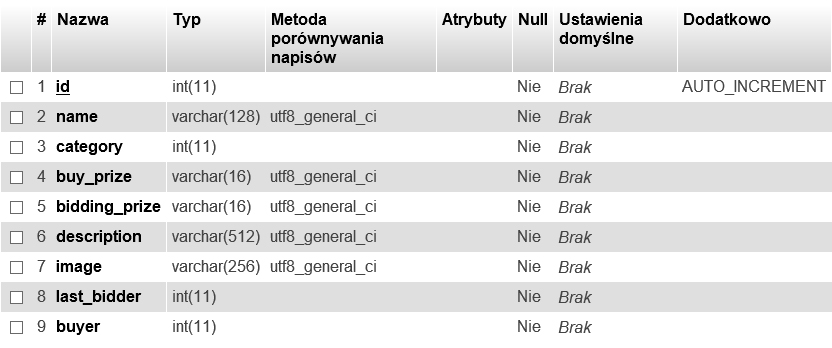
\includegraphics[width=12cm]{images/auctions.jpg}
		\caption{Tabela auctions}
	\end{figure}
	
	Struktura tabeli \emph{categories}:
	
	\begin{figure}[h]
		\centering
		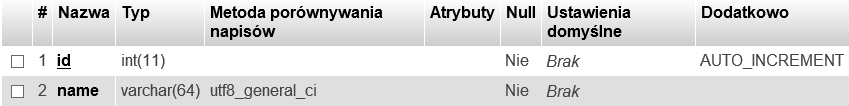
\includegraphics[width=12cm]{images/categories.jpg}
		\caption{Tabela categories}
	\end{figure}
	
	Struktura tabeli \emph{comments}:
	
	\begin{figure}[h]
		\centering
		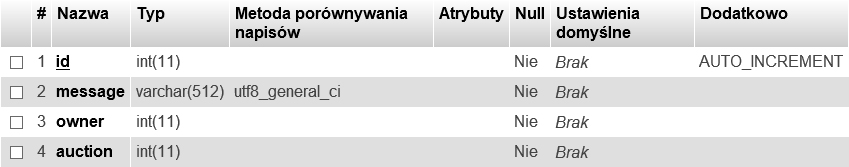
\includegraphics[width=12cm]{images/comments.jpg}
		\caption{Tabela comments}
	\end{figure}
	
	Struktura tabeli \emph{messages}:
	
	\begin{figure}[h]
		\centering
		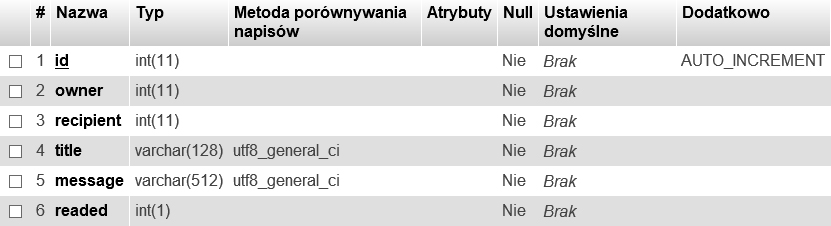
\includegraphics[width=12cm]{images/messages.jpg}
		\caption{Tabela messages}
	\end{figure}
	
	Struktura tabeli \emph{users}:
	
	\begin{figure}[h]
		\centering
		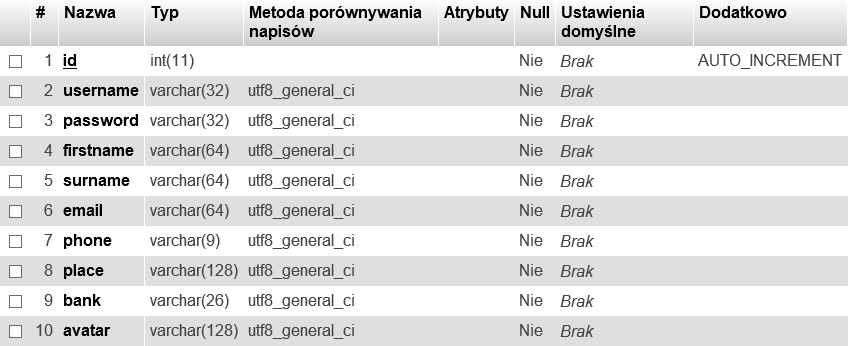
\includegraphics[width=12cm]{images/users.jpg}
		\caption{Tabela users}
	\end{figure}
	
	\paragraph{Tytuł zadania.} Rejestracja;
	\subparagraph{Wykonawca.} Kuba Niewczas;
	\subparagraph{Realizacja.} Tworząc skrypt rejestacji przypisałem pobrane dane z formularza metodą \emph{POST} do zmiennych. W postaci zapytania \emph{MySQL} dane zawarte w zmiennych będą dodawane do bazy danych do tabeli \emph{users}. Zadanie nie wymagało zbyt wielkiego poświęcenia czasu gdyż składa się tylko z paru operacji.
	
	\paragraph{Tytuł zadania.} Weryfikacja danych;
	\subparagraph{Wykonawca.} Kuba Niewczas;
	\subparagraph{Realizacja.} Do wcześniejszego zadania \textbf{Rejestracja} dodałem warunki, które muszą być spełnione aby użytkownik mógł założyć swoje konto. Użyłem zmiennych, które zostały zadeklarwane w bazowym zadaniu. Na początku wykonałem dwa zapytania do bazy danych aby sprawdzić czy wpisany \emph{login oraz hasło} istnieją już w bazie - jeśli tak to zwracana jest wiadomość, że konto na takie dane już istnieje. Lista warunków z backlogu została oskryptowana, w przypadku gdy skrypt ustali, że użytkownik popełnił błąd zostanie mu zwrócona informacja w postaci wyskakującego okienka \emph{JavaScriptu}.
	
	\subsection{Sprint Review/Demo}
	Sprint został zakończony powodzeniem. Wszystkie załozone zadania zostały zrealizowane w ustalonym czasie. Zostały zrealizowane następujące zadania:
	
\begin{itemize}
\item Została założona baza danych oparta na Środowisku bazodanowym MySQL, baza danych (która została uzupełniona w odpowiednie wiersze) umożliwia użytkownikowi założenie konta oraz logowanie się na stronie.
\item Został utworzony formularz który ma na celu umożliwienie logowania się na swoje konto.

\item Została stworzona weryfikacja danych wprowadzanych przy Rejestracji oraz Logowaniu: mająca na celu sprawdzić poprawność wpisanych danych przez użytkownika, w przypadku kiedy użytkownik nie wprowadzi poprawnych danych wyświetli się komunikat w postaci alertu podający w którym miejscu użytkownik popełnił jakiś błąd, oraz jaki to był błąd.

\item Formularz sprawdza czy istnieje w bazie danych podany login oraz hasło i czy te dane są przypisane tylko do jednego użytkownika. Została zaimplementowana wiadomość zwrotna gdy użytkownik wpisze złe dane “nie ma takiego rekordu w bazie danych bądź hasło nie pasuje do loginu” jeśli dane są poprawne wyświetli się komunikat “logowanie powiodło się” i użytkownik zostanie przekierowany na główna stronę serwisu.

\end{itemize}

	\section{Sprint 2}
	
	\subsection{Cel} Celem drugiego sprintu jest utworzenie "Panelu konta", który ma ułatwić użytkownikowi zarządzanie danymi oraz w przyszłości aukcjami. Zostanie również stworzona wyszukiwarka która w przyszłości pozowoli wyszukać konkretne produkty.
	
	\subsection{Sprint Planning/Backlog}
	
	\paragraph{Tytuł zadania.} Pasek nawigacji;
	\begin{itemize}
		\item Estymata: S;
	\end{itemize}
	
	\paragraph{Tytuł zadania.} Zmiana danych;
	\begin{itemize}
		\item Estymata: S;
	\end{itemize}
	
	\paragraph{Tytuł zadania.} Wyszukiwarka;
	\begin{itemize}
		\item Estymata: M;
	\end{itemize}
	
	\paragraph{Tytuł zadania.} Panel konta;
	\begin{itemize}
		\item Estymata: M;
	\end{itemize}
	
	\subsection{Realizacja}
	
	\paragraph{Tytuł zadania.} Pasek nawigacji;
	\subparagraph{Wykonawca.} Kuba Niewczas;
	\subparagraph{Realizacja.} Pasek nawigacji stworzyłem u góry ekranu, zablokowałem go w tym miejscu na stałe używając wbudowanej opcji Bootstrap'a (framework, który używamy w projekcie) - \verb|navbar-fixed-top|, przez co będzie podążał razem ze stroną podczas scrollowania. Wygląd całego paska stworzyłem w \emph{CSS} - szerokość dopasowywuje się do wielkości ekranu, na którym wyświetlana jest strona a sama zawartość paska jest umiejscowiana od środka.
	
	\paragraph{Tytuł zadania.} Wyszukiwarka;
	\subparagraph{Wykonawca.} Kuba Niewczas;
	\subparagraph{Realizacja.} Obecne zadanie jest kontynuacją poprzedniego zadania \emph{(tj. pasek nawigacji)}. Na pasku dodałem jeden większy input formularza z wiadomością podpowiadającą do czego służy (gdy użytkownik napiszę jakieś hasło w inpucie wiadomość domyślna automatycznie się usuwa). Wpisane przez osobę hasło pobieram metodą \emph{POST} oraz przepuszczam przez funkcję \emph{htmlspecialchars()}, zwróconą wartość umieściłem w zapytaniu MySQL w postaci (\verb|[...]name LIKE %zmienna%[...]|). Ostatnim etapem jest przeniesienie osoby na podstronę, na której są wypisane aukcje, które zawierają ciąg wpisany w wyszukiwarkę.
	
	\paragraph{Tytuł zadania.} Panel konta;
	\subparagraph{Wykonawca.} Kuba Niewczas;
	\subparagraph{Realizacja.} Zadanie jest kontynuacją poprzedniego zadania \emph{(tj. pasek nawigacji)}. W przypadku gdy osoba nie jest zalogowana na swoję konto stworzyłem napis po prawej stronie wyszukiwarki \emph{Moje konto}, w które jeśli klikniemy pojawi się kwadracik a w nim mini-menu \emph{(tj. zarejestruj się oraz zaloguj się)} - po kliknięciu zostajemy przekierowani na odpowiednie podstrony. W przypadku gdy osoba jest zalogowana to obok wyszukiwarki wyświetla się awatar osoby w kształcie okręgu, który również można kliknąc i pojawi się mini-menu \emph{(tj. edytuj dane, moje aukcje, historia zakupów, wyloguj)} - podobnie jak wyżej, po kliknięciu w menu skrypt przekierowywuje nas na odpowiednią podstronę.
	
	\paragraph{Tytuł zadania.} Zmiana danych;
	\subparagraph{Wykonawca.} Damian Klimek;
	\subparagraph{Realizacja.} Obecne zadanie jest uzupełnieniem do zadania \emph{Panel konta}. Polegało na stworzeniu podstrony do "Zmień dane" w zakładce Panelu konta. Został stworzony formularz z danymi (tj. imie, nazwisko, email, miejscowosc, numer telefonu, numer konta bankowego, hasło oraz avatar) który pobiera dane z tabeli \emph{users}, a następnie umożliwia zmianę ich poprzez wysłanie zapytania \emph{UPDATE} do bazy danych. Został również dodany przycisk submit (Wyślij).
	
	\subsection{Sprint Review/Demo}
	
	Sprint został zakończony powodzeniem. Wszystkie załozone zadania zostały zrealizowane w ustalonym czasie. Zostały zrealizowane następujące zadania:
	
\begin{itemize}

\item Został utworzony pasek nawigacyjny umożliwiający użytkownikowi nawigacje po serwisie.
\item Został utworzony panel konta w którym możemy zarządzać swoim kontem oraz zmienić dane.
\item Została utworzona wyszukiwarka na pasku nawigacyjnym dzięki której możemy wyszukać interesującą nas aukcje.

\end{itemize}
	
	\section{Sprint 3}
	
	\subsection{Cel} Celem trzeciego sprintu jest umożliwienie zalogowanemu użytkownikowi dodawania aukcji oraz jej edytowania. Zostanie również stworzona lista dostępnych aukcji oraz formularz aukcyjny.
	
	\subsection{Sprint Planning/Backlog}
	
	\paragraph{Tytuł zadania.} Dodanie aukcji;
	\begin{itemize}
		\item Estymata: L;
	\end{itemize}
	
	\paragraph{Tytuł zadania.} Lista aukcji;
	\begin{itemize}
		\item Estymata: M;
	\end{itemize}
	
	\paragraph{Tytuł zadania.} Formularz aukcyjny;
	\begin{itemize}
		\item Estymata: S;
	\end{itemize}
	
	\paragraph{Tytuł zadania.} Edytowanie aukcji;
	\begin{itemize}
		\item Estymata: M;
	\end{itemize}
	
	\subsection{Realizacja}
	
	\paragraph{Tytuł zadania.} Dodanie aukcji;
	\subparagraph{Wykonawca.} Kuba Niewczas;
	\subparagraph{Realizacja.} Z poziomu panelu konta użytkownika (kliknięcie w avatar na pasku nawigacji po czym wybranie pozycji \emph{dodaj aukcję}) następuję przekierowanie na nową podstronę. Jeśli użytkownik nie jest zalogowany na swoje konto dostaję wiadomość, iż nie posiada dostępu na przebywanie na podstronie i zostaje wyświetlona mu strona głowna. Stworzyłem zapytanie, które tworzy nowy rekord w bazie \emph{auctions}.
	
	\paragraph{Tytuł zadania.} Formularz aukcyjny;
	\subparagraph{Wykonawca.} Kuba Niewczas;
	\subparagraph{Realizacja.} Obecne zadanie jest rozszerzeniem powyższego zadania \emph{(tj. dodanie aukcji)}. Stworzyłem formularz z następującymi danymi \emph{(nazwa aukcji, kategoria, opis aukcji, zdjęcie przedmiotu, cena kup teraz, cena licytacji)}. Dane pobieram metodą POST oraz przypisuję je do zmiennych a następnie lądują one do zapytania. 
	
	\paragraph{Tytuł zadania.} Lista aukcji;
	\subparagraph{Wykonawca.} Damian Klimek;
	\subparagraph{Realizacja.} Została stworzona lista aukcji, która jest pobierana z bazy danych (tabela \emph{auctions}) oraz wyświetlana na stronie głównej dla wszystkich użytkowników, lista ta: wyświetla obrazek aukcji, nazwę aukcji oraz jej cenę. W przyszłości umożliwi przejście do danej aukcji.
	
	\paragraph{Tytuł zadania.} Edytowanie aukcji;
	\subparagraph{Wykonawca.} Tomasz Zabrzewski;
	\subparagraph{Realizacja.} Zadanie to polegało na stworzeniu podstrony z możliwością edycji aukcji tylko dla osoby która tą aukcje wystawiła. Został stworzony formularz z danymi (tj. nazwa, kategoria, cena kupna, cena licytacji, opis, zdjęcie) który pobiera dane z tabeli \emph{auctions}, a następnie umożliwia zmianę ich poprzez wysłanie zapytania \emph{UPDATE} do bazy danych.
	
	\subsection{Sprint Review/Demo}
	Sprint został zakończony powodzeniem. Wszystkie załozone zadania zostały zrealizowane w ustalonym czasie.
	
	\section{Sprint 4}
	
	\subsection{Cel} Celem czwartego sprintu jest m.in. umożliwienie właścicielowi danej aukcji usunięcia jej, dodanie możliwości grupowania aukcji wg. kategori. Będzie teraz można wejść w daną aukcję i zapoznać się z dokładną jej treścią, a następnie ją kupić. Zostanie również udostępniona opcja komentowania wybranych aukcji.
	
	\subsection{Sprint Planning/Backlog}
	
	\paragraph{Tytuł zadania.} Usuwanie aukcji;
	\begin{itemize}
		\item Estymata: L;
	\end{itemize}
	
	\paragraph{Tytuł zadania.} Kategorie;
	\begin{itemize}
		\item Estymata: M;
	\end{itemize}
	
	\paragraph{Tytuł zadania.} Kupowanie przedmiotu;
	\begin{itemize}
		\item Estymata: S;
	\end{itemize}
	
	\paragraph{Tytuł zadania.} Komentarze;
	\begin{itemize}
		\item Estymata: M;
	\end{itemize}
	
	\paragraph{Tytuł zadania.} Podgląd aukcji;
	\begin{itemize}
		\item Estymata: M;
	\end{itemize}
	
	\subsection{Realizacja}	
	
	\paragraph{Tytuł zadania.} Usuwanie aukcji;
	\subparagraph{Wykonawca.} Damian Klimek
	\subparagraph{Realizacja.} Zadanie to polegało na stworzeniu podstrony z możliwością usunięcia aukcji tylko dla osoby która tą aukcje wystawiła, a następnie umożliwia zmianę ich poprzez wysłanie zapytania \emph{DELETE} do bazy danych.
	
	\paragraph{Tytuł zadania.} Kategorie;
	\subparagraph{Wykonawca.} Damian Klimek
	\subparagraph{Realizacja.} Zostały stworzone kategorie, które pobierają się z bazy danych z tabeli \emph{categories}. Kategorie te są wyświetlane na stronie głównej obok listy aukcji, po kliknięciu w wybraną kategorię następuje przekierowanie na podstronę z aukcjami przypisanymi do danej kategorii.
	
	
	Każda osoba odwiedzająca serwis powinna mieć dostępny pasek boczny z dostępnymi kategoriami. Kategorie powinny być wczytywane z bazy danych z tabeli \emph{categories}, w postaci odsyłacza który umożliwi przekierowanie osoby na podstronę wybranej kategorii, gdzie zostaną wyświetlone wszystkie aukcje należące do danej kategorii. 
	
	
	\paragraph{Tytuł zadania.} Podgląd aukcji;
	\subparagraph{Wykonawca.} Kuba Niewczas
	\subparagraph{Realizacja.} Stworzyłem oddzielną podstronę, na której widnieją wszystkie informację związane z daną aukcją. Każda osoba ma dostęp do tej podstrony. Dane wyświetlają się w postaci tabelki. 
	
	\paragraph{Tytuł zadania.} Kupowanie przedmiotu;
	\subparagraph{Wykonawca.} 
	\subparagraph{Realizacja.}
	
	\paragraph{Tytuł zadania.} Komentarze;
	\subparagraph{Wykonawca.} Kuba Niewczas
	\subparagraph{Realizacja.} Zadanie jest rozszerzeniem do zadania \emph{Podgląd aukcji}. Pod podglądem aukcji stworzyłem sekcję komentarzy, które są widoczne dla każdej osoby (zalogowanej lub niezalogowanej). Poniżej komentarzy znajduje się \emph{textarea}, z której dane pobierane są metodą POST a następnie wysyłane w postaci zapytania do bazy do tabeli \emph{comments}. Komentarz jest przypisany do osoby, która go wysyła (w podglądzie komentarza na stronie aukcji widnieje avatar oraz nazwa użytkownika). Dodawać komentarze mogą tylko osoby zalogowane.
	
	\subsection{Sprint Review/Demo}
	Sprint został zakończony częściowym powodzeniem. Nie wszystkie załozone zadania zostały zrealizowane w ustalonym czasie. Zadania które zostały w dniu dzisiejszym (09-01-2018) zaprezentowane to:
	
\begin{itemize}

\item Zostało utworzone usuwanie aukcji, dzięki któremu można usunąć swoją aukcję.
\item Został utworzony podgląd aukcji, w którym można zobaczyć wszystkie informacje związane z daną aukcją.
\item Został utowrzony panel kategorii dzięki któremu możemy przejść do interesującej nas kategorii.
\item Została stworzona sekcja komentarzy, dzięki której możemy jako zalogowany użytkownik dodawać komentarze pod aukcją. W czasie sprint review został zauważony problem z dodawaniem komenatrzy, który został rozwiązany po dokładnym przeanalizowaniu kodu.
\end{itemize}
	
Zadania niezrealizowane, które przechodzą na następny sprint to:

\begin{itemize}

\item Wystąpiły niespodziewane komplikacje z kupowaniem przedmiotu. 

\end{itemize}


\section{Sprint 5}
	
	\subsection{Cel} Celem piątego sprintu jest umożliwienie wysyłania wiadomości, możliwość wyświetlenia wszystkich swoich aukcji na stronie, kupowanie przedmiotu oraz otrzymanie informacji zwrotnej po kupieniu przedmiotu.
	
	\subsection{Sprint Planning/Backlog}
	
	\paragraph{Tytuł zadania.} Wiadomości;
	\begin{itemize}
		\item Estymata: L;
	\end{itemize}
	
	\paragraph{Tytuł zadania.} Informacja zwrotna;
	\begin{itemize}
		\item Estymata: M;
	\end{itemize}
	
	\paragraph{Tytuł zadania.} Kupowanie przedmiotu;
	\begin{itemize}
		\item Estymata: XL;
	\end{itemize}
	
	\paragraph{Tytuł zadania.}Moje aukcje;
	\begin{itemize}
		\item Estymata: L;
	\end{itemize}
	
	\subsection{Realizacja}
	
	\paragraph{Tytuł zadania.} Wiadomości
	\subparagraph{Wykonawca.} Kuba Niewczas
	\subparagraph{Realizacja.} Zadanie to polegało na utworzeniu panelu, w którym można wysłać wiadomość do innego użytkownika serwisu w celu skontaktowania się z nim. W panelu należy podać tytuł, odbiorcę oraz treść wiadomości, aby móc ją wysłać.
	
	\paragraph{Tytuł zadania.} Informacja zwrotna
	\subparagraph{Wykonawca.} Kuba Niewczas
	\subparagraph{Realizacja.} W tym zadaniu została utworzona informacja zwrotna, która jest wysyłana zarówno do kupującego jak i sprzedającego. Wiadomość ta zawiera informacje dotyczące aukcji. W chwili dokonania zakupu, kupującemu wyświetli się powiadomienie o tym, że zakupił wybrany przez siebie przedmiot. Natomiast sprzedającemu wyświetli się komunikat, że wystawiony przez niego przedmiot został sprzedany.
	
	\paragraph{Tytuł zadania.} Kupowanie przedmiotu
	\subparagraph{Wykonawca.} Kuba Niewczas
	\subparagraph{Realizacja.} Została dodana możliwość kupienia przedmiotu przez użytkowników zalogowanych na stronie. Zalogowani użytkownicy mogą kupić przedmiot używając opcji „kup teraz”. Po zakupie przedmiotu, zostaje on usunięty z listy aukcji oraz zostaje wysłana informacja zwrotna zarówno do kupującego jak i sprzedającego.

	\paragraph{Tytuł zadania.} Moje aukcje
	\subparagraph{Wykonawca.} Kuba Niewczas
	\subparagraph{Realizacja.} Utworzone zostało menu, w którym zalogowanemu użytkownikowi wyświetlają się wszystkie przedmioty wystawione przez niego na aukcję. Dostęp do tego menu ma tylko osoba, która wystawiła te aukcje. Wyświetlają się tam informacje o tytule aukcji, cenie jak i dacie wystawienia każdego przedmiotu na aukcję.
	
	\subsection{Sprint Review/Demo}
	
	\begin{itemize}

\item Została stworzona możliwość kupowania przedmiotów, użytkownik może kupować interesujące go przedmioty poparzez opcje kup teraz.
\item Została stworzona informacje zwrotna, osobie kupujące wyświetla się informacja o kupieniu przedmiotu, a osobie sprzedajacej wyświetla się informacja o sprzedaniu swojego przedmiotu.
\item Została stworzona możliwość wglądu do swoich aukcji, które zostają wystawione na stronie.
\item Została stworzona możliwość przesyłania wiadomości między zalogowanymi użytkownikami serwisu.

\end{itemize}
	
	\begin{thebibliography}{9}
		
		\bibitem{Cov} S. R. Covey, {\em 7 nawyków skutecznego działania}, Rebis, Poznań, 2007.
		
		\bibitem{Oet} Tobias Oetiker i wsp., Nie za krótkie wprowadzenie do systemu \LaTeX  \ $2_\varepsilon$, \url{ftp://ftp.gust.org.pl/TeX/info/lshort/polish/lshort2e.pdf}
		
		\bibitem{SchSut} K. Schwaber, J. Sutherland, {\em Scrum Guide}, \url{http://www.scrumguides.org/}, 2016.
		
		\bibitem{apr} \url{https://agilepainrelief.com/notesfromatooluser/tag/scrum-by-example}
		
		\bibitem{us} \url{https://www.tutorialspoint.com/scrum/scrum_user_stories.htm}
		
	\end{thebibliography}
	
\end{document}
